\documentclass[12pt,]{article}
\usepackage{lmodern}
\usepackage{amssymb,amsmath}
\usepackage{ifxetex,ifluatex}
\usepackage{fixltx2e} % provides \textsubscript
\ifnum 0\ifxetex 1\fi\ifluatex 1\fi=0 % if pdftex
  \usepackage[T1]{fontenc}
  \usepackage[utf8]{inputenc}
\else % if luatex or xelatex
  \ifxetex
    \usepackage{mathspec}
  \else
    \usepackage{fontspec}
  \fi
  \defaultfontfeatures{Ligatures=TeX,Scale=MatchLowercase}
\fi
% use upquote if available, for straight quotes in verbatim environments
\IfFileExists{upquote.sty}{\usepackage{upquote}}{}
% use microtype if available
\IfFileExists{microtype.sty}{%
\usepackage{microtype}
\UseMicrotypeSet[protrusion]{basicmath} % disable protrusion for tt fonts
}{}
\usepackage[margin=1in]{geometry}
\usepackage{hyperref}
\hypersetup{unicode=true,
            pdftitle={Smaller organisms are less strongly structured by environmental variation},
            pdfauthor={A. Andrew M. MacDonald, Vinicius F. Farjalla, Flavia Lima, Diane S. Srivastava},
            pdfborder={0 0 0},
            breaklinks=true}
\urlstyle{same}  % don't use monospace font for urls
\usepackage{longtable,booktabs}
\usepackage{graphicx,grffile}
\makeatletter
\def\maxwidth{\ifdim\Gin@nat@width>\linewidth\linewidth\else\Gin@nat@width\fi}
\def\maxheight{\ifdim\Gin@nat@height>\textheight\textheight\else\Gin@nat@height\fi}
\makeatother
% Scale images if necessary, so that they will not overflow the page
% margins by default, and it is still possible to overwrite the defaults
% using explicit options in \includegraphics[width, height, ...]{}
\setkeys{Gin}{width=\maxwidth,height=\maxheight,keepaspectratio}
\IfFileExists{parskip.sty}{%
\usepackage{parskip}
}{% else
\setlength{\parindent}{0pt}
\setlength{\parskip}{6pt plus 2pt minus 1pt}
}
\setlength{\emergencystretch}{3em}  % prevent overfull lines
\providecommand{\tightlist}{%
  \setlength{\itemsep}{0pt}\setlength{\parskip}{0pt}}
\setcounter{secnumdepth}{0}
% Redefines (sub)paragraphs to behave more like sections
\ifx\paragraph\undefined\else
\let\oldparagraph\paragraph
\renewcommand{\paragraph}[1]{\oldparagraph{#1}\mbox{}}
\fi
\ifx\subparagraph\undefined\else
\let\oldsubparagraph\subparagraph
\renewcommand{\subparagraph}[1]{\oldsubparagraph{#1}\mbox{}}
\fi

%%% Use protect on footnotes to avoid problems with footnotes in titles
\let\rmarkdownfootnote\footnote%
\def\footnote{\protect\rmarkdownfootnote}

%%% Change title format to be more compact
\usepackage{titling}

% Create subtitle command for use in maketitle
\newcommand{\subtitle}[1]{
  \posttitle{
    \begin{center}\large#1\end{center}
    }
}

\setlength{\droptitle}{-2em}
  \title{Smaller organisms are less strongly structured by environmental
variation}
  \pretitle{\vspace{\droptitle}\centering\huge}
  \posttitle{\par}
  \author{A. Andrew M. MacDonald, Vinicius F. Farjalla, Flavia Lima, Diane S.
Srivastava}
  \preauthor{\centering\large\emph}
  \postauthor{\par}
  \date{}
  \predate{}\postdate{}

\usepackage{lineno}
\linespread{2}
\linenumbers
%\usepackage{mathptmx}
\usepackage[document]{ragged2e}

\begin{document}
\maketitle

\subsection{Introduction}\label{introduction}

One of the most profound differences between organisms is their body
size. Small and large organisms can differ in population size, growth
rates, morphological complexity, genome size, and modes of dispersal.
This scaling of biological processes with organism size has often been
used to explain differences in the spatial distribution of small and
large organisms. Microscopic organisms such as bacteria and plankton are
often globally distributed, while larger organisms have more
geographically restricted distributions (Fenchel and Finlay 2004). Even
within landscapes, there is some evidence that the occurrence of
microscopic organisms responds less to environmental gradients than does
the occurrence of larger organisms (Fierer et al. 2011; Farjalla et al.
2012; Louca et al. 2016). However, while such differences in
distribution suggest that the suite of processes underlying community
assembly differ between small and large organisms, it is difficult to
determine which process is driving this difference. There are at least
two possible mechanisms that may make communities of smaller organisms
more widely distributed. First, smaller organisms could have larger
environmental tolerances, allowing them to occupy broader fundamental
niches. Second, smaller organisms could have greater dispersal
abilities, allowing them to reach more habitats.

Smaller organisms may have broader environmental tolerances for several
reasons. First, their small body size allows habitat heterogeneity to
affect them at very small scales: smaller organisms are able to find
tolerable microhabitats, while organisms that experience the environment
at a coarser grain may not detect a similar variation in the
environment. This biological difference between small and large
organisms can be compounded by the macroscopic grain at which organisms
are typically observed by researchers, which averages over any
microscopic-scale variation in distribution (Wiens 1989). Secondly,
single-celled organisms may be able to use multiple carbon sources
(Langenheder and Ragnarsson 2007) allowing them to survive in a greater
range of habitats. Very small organisms are also more likely to possess
resting stages when a habitat is unfavorable (e.g.~cysts for protists,
tun state for tardigrades) or to propagate by means of a resistant life
history stage such as spores. At the population level, small organisms
may persist in a habitat if they are able to adapt to rapidly adapt to
local conditions by virtue of their short generation times and high
population sizes. In the case of bacteria, genetic adaptation can also
involve lateral gene transfer between lineages (Ochman et al. 2000).

Alternatively, small organisms may be widely distributed because they
are able to get to more places faster. There is substantial evidence
that microscopic organisms such as bacteria, viruses, protists and
plankton may be able to disperse further than larger organisms; amongst
these microscopic organisms, the smallest disperse the furthest (De Bie
et al. 2012). This is the reasoning behing the classic ``everything is
everywhere and the environment selects'' hypothesis of Baas Becking
(1934), which suggests that smaller organisms are not limited by
dispersal barriers or distance but instead are found globally, emerging
from resistant stages in favorable environments (Huszar et al. 2015).
Many bacteria and zooplankton have passive dispersal, traveling long
distances by wind or water currents, or by phoresy. In contrast, larger
animals (but not larger plants) usually have active dispersal; for
example, adult insects actively choose sites to oviposit. At the scale
of landscapes, active dispersal could result in a close association
between distribution and environmental variables, assuming that active
dispersal behaviour is adapted to maximize fitness. However, at
continental and global scales, the limited distances covered by active
dispersers might prevent larger animals from reaching suitable places.
This would weaken the association between environment and distribution
for larger animals.

It has been difficult to determine whether differences in distribution
between small and large organisms is caused by differences in the
strength of environmental filtering or dispersal limitation. There are
three reasons for this. First, the distribution of micro-and macroscopic
organisms has rarely been compared within the same system. This creates
a problem of scale, with studies of many macroscopic organisms occurring
on much smaller spatial scales than those of microscopic organisms.
Second, when we rely on observational data alone, we have a limited
ability to infer environmental filtering. This is because environment,
space and dispersal are often correlated. Previous researchers have used
variance partitioning to separate the effects of environment from space,
but this approach has limitations (Gilbert and Bennett 2010). For
example, Smith and Lundholm (2010) found that spatially-correlated
dispersal contributed to both spatial and environmental partitions of
variance in community composition. Third, dispersal limitation and
environmental filtering can mask each other. A species can only be
filtered by a site's environment when it can reach the site, so a
community experiencing equally strong dispersal and environmental
limitation can may show mainly the former in variance partitioning
(Smith and Lundholm 2010; De Bie et al. 2012). A special case of this
problem occurs when an actively-dispersing species is not found in a
site. It is impossible to determine if this is because the environment
makes dispersal unlikely or establishment unlikely. For example, an
insect larva may be missing from a location because its parent was
deterred from ovipositing in the environment or because the larvae could
not withstand the environment. An experiment that removes dispersal
limitation for all organisms is therefore a stronger test of the
relative effects of environment on species composition. We are aware of
no study that experimentally removes dispersal limitation for both
micro- and macroscopic organisms in the same system, simultaneously, to
reveal environmental filtering. We conducted such an experiment, using
patchy natural mesocosms (bromeliad phytotelmata) as model communities.

\subsubsection{Study system}\label{study-system}

Tank bromeliads (Bromeliaceae) retain rainwater in their bowl-like
leaves, creating patches of aquatic habitat throughtout Neotropic
forests. These small patches of habitat are inhabited by many species of
macroinvertebrates, especially insects (Frank and Lounibos 2009),
zooplankton (Petermann et al. 2015), and bacteria (Haubrich et al. 2009;
Louca et al. 2017). Importantly, different species of bromeliad grow in
different habitats, and this habitat variation is correlated with
differences among their communities (Marino et al. 2013). Previous
observations in this system show that this environmental variation is
closely associated with variation in macroinvertebrate composition,
weakly associated with variation in zooplankton communities and almost
uncorrelated with variation in bacterial communities (Farjalla et al.
2012).

Here we provide a robust test of the strength of environmental filtering
for these three organism groups, which differ widely in size:
macroinvertebrates (large, 5 to 50 mm), zooplankton (intermediate, 2 x
10\textsuperscript{-1} to 2 mm) and bacteria (small, 5 x
10\textsuperscript{-3} to 5 x 10\textsuperscript{-4} mm). In this test
we dispersed all species to all habitats, and examined whether the
original habitat-based patterns in composition re-emerged. We predicted:

\begin{enumerate}
\def\labelenumi{\arabic{enumi}.}
\tightlist
\item
  If environmental filtering, but not dispersal limitation, increases
  with organism size, we would predict that habitat would affect the
  composition of communities of large-bodied organisms more than those
  of small-bodied organisms (Figure 1a). 
\item
  If instead only dispersal limitation increased with organism size, we
  would expect that any apparent effect of habitat on community
  composition was an artifact of spatial autocorrelation and would be
  erased by our removal of dispersal limitation (Figure 1b).
\item
  If both environmental filtering and dispersal limitation increased
  with organism size, we would predict an intermediate scenario (Figure
  1c).
\end{enumerate}

\subsection{Methods}\label{methods}

\subsubsection{Study site}\label{study-site}

We performed this experiment in the same location and along the same
gradient of environmental variation (bromeliad species in different
habitats) as Farjalla et al. (2012). Both their study and ours took
place in the Parque Nacional de Jurubatiba, Northeast Rio de Janeiro
state, Brazil (\(22^{\circ}\) S \(41^{\circ}\) W). The environmental
gradient in this ecosystem is twofold -- three different species of
bromeliad, which differ also in their preferred level of exposure to
sunlight: \emph{Aechmea nudicaulis} (full sun habitats), \emph{Vriesea
neoglutinosa} (partial shade), and \emph{Neoregelia cruenta} (full
shade).

\subsubsection{Experimental design}\label{experimental-design}

For each of five temporal blocks, we collected and sampled the
macroinvertebrates, zooplankton and bacteria of two bromeliads of each
of the three species. We then homogenized the communities of all six
bromeliads as described shortly (Figure 2). Our goal was to create
identical starting community composition for all bromeliads within a
block. Variation between blocks in starting community composition is
thus included in the random effect of blocks. We created five blocks in
this experiment between 27 March 2013 and 03 April 2013.

Our experimental setup consisted of three steps (Figure 2): collection
of original communities from bromeliads, homogenization of communities,
and assembly of this homogenized community in each of the original (now
empty) bromeliads. \textbf{Original communities}: We sampled the
zooplankton and bacteria communities by collecting water samples from
each bromeliad: 100ml for zooplankton, 50ml for bacteria; this sample
volume was based on previous studies (Farjalla et al. 2012). Zooplankton
were collected by filtering on \(50\mu\)m Nytex mesh and fixed in 5\%
buffered formalin. This fixed solution was then diluted to 20 ml, and a
1 ml subsample taken for analysis. Zooplankton were identified to the
lowest taxonomic unit possible (species in most cases, except for
bdelloid rotifers and harpaticoid copepods, identified to class and
order, respectively). Bacteria were collected by taking 100ml of
filtrate from the zooplankton sample and filtering it a second time on
\(0.2\mu\)m nitrocellulose filters (Whatman filter paper) which were
then stored at -20C. We measured bacterial community composition using
denaturing gradient gel electrophoresis (DGGE, Muyzer et al. (1993)).
This technique measures an approximation of bacterial diversity in the
form of Operational Taxonomic Units (OTUs). Although this yieds fairly
coarse-level separation of taxonomic groups, we used this method to be
able to replicate the original results of Farjalla et al. (2012). We
demonstrate later that our results are qualitatively similar to that
obtained by marker gene sequencing (Louca et al. 2016). We sampled
macroinvertebrates by thoroughly rinsing each bromeliad and filtering
the water through 1mm and 180μm mesh. These mesh sizes have been shown
to separate macroinvertebrates from both coarse detritus and fine
particulate organic matter, facilitating their collection (Romero and
Srivastava 2010). We identified macroinvertebrates to morphospecies.
\textbf{Homogenized communities}: We created homogenized communities of
zooplankton and microbes by mixing an equal volume of filtered tank
water from each of the six bromeliads in a block (approximately 100ml
plant\textsuperscript{-1}), then adding this mixture to all bromeliads.
To create homogenized communities of macroinvertebrates, we divided
individuals of all species equally among the six bromeliads in each
block. \textbf{Community assembly in bromeliads}: We emptied bromeliads
by washing them thoroughly, hanging them upside down to dry for at least
24 hours and then rinsing each plant with 70\% ethanol. We confirmed
that this technique removed all invertebrates and most detritus by
dissecting an empty bromeliad. Any coarse detritus found in the
bromeliads was similarly cleaned, frozen and thawed (to kill any eggs or
resting stages of macroinvertebrates). Bromeliads were placed in a local
habitat similar to their original location: \emph{Neoregelia} in shade,
\emph{Aechmea} in full sun and \emph{Vriesea} in marginal habitat. We
then added the starting communities of macroinvertebrates, zooplankton
and bacteria.

Bromeliads are an open system, characterized by continual colonization
and emergence. Both of these processes are problematic for our question.
If we were to allow colonization it could swamp any changes in our
starting community composition. Conversely, if we allowed the experiment
to continue for too long any macroinvertebrates with complex life cycles
would emerge, leaving us with no community to sample (Lecraw et al.
2014). We took two steps to make sure that our treatment effects were
not affected by colonization or excessive emergence. To prevent
colonization we surrounded bromeliads with mosquito netting (mesh size
approx. 1.5 mm). To prevent emergence we ended our experiment after 12
days, based on the results of a pilot study that confirmed that this was
sufficient time for communities to change, but not so long that
bromeliads became empty of organisms

\subsubsection{Analyses}\label{analyses}

We distinguished between our three predictions (Figure 1) with a
permutational ANOVA (PERMANOVA), which measures the amount of difference
in community composition between treatment groups and compares this to
the expected distribution under a null hypothesis of no treatment
effects. In each PERMANOVA we used block as an error stratum, meaning
that permutations were performed within blocks. We repeated this
analysis for all three organism types, and at both the beginning and end
of the experiment. We interpreted the R\textsuperscript{2} value of this
PERMANOVA as a metric of the strength of habitat filtering (Figure 1).
Our hypothesis predicted that R\textsuperscript{2} values should
increase from smaller to larger organism types. However, because we
sampled each of these groups with different techniques, and collected
different types of data (e.g.~abundance data for macroinvertebrates,
presence/absence for bacterial OTUs) we may observe different
R\textsuperscript{2} values through statistical, not biological,
processes. Therefore we tested a pattern of increasing
R\textsuperscript{2} against the increase that would be expected under
the null hypothesis of no difference in environmental filtering. We
first quantified the upward trend with the slope of a linear regression
of R\textsuperscript{2} as a function of approximate organism size
(bacteria = 0.04mm, zooplankton = 0.5mm, macroinvertebrates = 5mm). To
generate our null distribution, we generated a random permutation of the
environmental variable (i.e.~bromeliad species). We used the same
permutation series for each organism type. We calculated the
standardized effect size (SES) of the observed slope (\(\beta\)) with
the equation

\[
\mbox{SES} = \frac{\beta_{\mbox{observed}} - \bar{\beta}_{\mbox{null}})}{\mbox{SD}(\beta_{\mbox{null}})}
\]

We calculated the null p-value as the proportion of null simulations
equal or greater to the observed slope. All statistical analyses were
conducted in R 3.2.3 (R Core Team 2015).

\subsection{Results}\label{results}

Both before and at the end of our experiment, bromeliad species identity
explains more variation in community composition of macroinvertebrates
than any other organism type, less for zooplankton and less still for
bacteria (Figure 3, Table 1). For all organism types, bromeliad species
explained less of the variation in composition at the end of the
experiment than before the homogenization. Note that, although the
sampling design (and therefore degrees of freedom) are identical for all
groups, the critical (alpha = 0.05) F-value for each organism group
differs because PERMANOVA p-values are calculated on a null distribution
generated by permuting samples among groups (species in our case).
Bacterial communities have many species and also high similarity among
communities (bromeliads), creating a null distribution with low mean and
small variance (and hence lower thresholds for significance). This
increases the power to detect habitat effects for bacteria, explaining
why this group has marginally significant effects of habitat despite
habitat explaining a tiny amount of total variation in composition.

So far, we have assessed the absolute effect of habitat filtering on
each organism group separately, but our goal was also to determine if
the strength of habitat filtering increases between the organism groups.
We therefore compared this pattern of increasing environmental effects
with a null model. First, we calculated the slope of the relationship
between the R\textsuperscript{2} value and approximate organism size. We
then generated null distributions by reshuffling bromeliad species
within blocks, using the same permutation across all organism types. We
found that the observed slope was much higher than the null simulations
for both initial (SES = 6.46, p = 0.002) and final (SES = 4.87, p =
0.002) sampling (499 simulations).

\subsection{Discussion}\label{discussion}

\subsubsection{Main findings}\label{main-findings}

Our study compared the response of macroinvertebrates, zooplankton and
bacterial communities to an identical environmental gradient. Our
initial sampling prior to the experimental manipulation found that the
correlation between environment and community composition is weakest for
bacteria, intermediate for zooplankton, and strongest for
macroinvertebrates (Figure 3). This observational pattern mirrors that
previously reported by Farjalla et al. (2012), confirming that the
observational pattern is robust to differences in field site and year.
However, this observed pattern may have been caused by differences among
the three organism types in the strength of environmental filtering or
environmentally-correlated dispersal, or both (Figure 1). We therefore
removed dispersal limitation among communities by homogenizing our
starting communities, and then returned communities to the same
environmental gradient to test whether pure environmental filtering was
sufficient to restore the initial pattern in distributions. Our results
are most consistent with environmental filtering increasing with
organism size (Fig 1a). Specifically, we found that the environment
created minimal differences in bacteria, weak differences in
zooplankton, and large differences in macroinvertebrates (Figure 3).

Our experimental manipulation suggests that environmental filtering is
stronger for larger than smaller organisms, and that this explains the
differences observed in the field between organismal groups. An increase
in environmental filtering with body size is most simply explained as a
contraction in the breadth of the fundamental niche as organism body
size increases. Farjalla et al. (2012) termed this hypothesis the
``size-plasticity hypothesis'' and, like us, related it to differences
in the distribution of bacteria, zooplankton and macroinvertebrates
between bromeliads. Studies of other groups of organisms across
environmental gradients within landscapes also show the same pattern of
increasing environmental determinism with body size. For example, along
mountainsides, elevation explains more variation in vascular plant
diversity than in bacteria (Bryant et al. 2008). In streams,
environmental variation also correlates more strongly with stream
invertebrate than bacterial composition (Wang et al. 2012). Similar
patterns are also found in a group of Finnish lakes, where Soininen et
al. (2013) analyzed the distribution of individual taxa rather than
organism groups. They found that models describing the distribution of
taxa in terms of the environment had greater predictive power for
zooplankton than phytoplankton than bacteria.

Interestingly, while this pattern of increasing environmental
determinism with body size is found frequently when multiple groups are
compared along the same small environmental gradient, this effect can be
absent (or even reversed) between studies or along regional spatial
scales. In a meta-analysis of 326 studies covering a broad range of
ecosystems and taxa, neither body size nor dispersal ability predicted
the strength of environment filtering for individual species (Soininen
2014). A study comparing various freshwater groups across all of Belgium
found that passively-dispersed organisms with larger propagules showed
\emph{less} environmental signal than those with small propagules,
probably because the positive association between organism size with
dispersal limitation masked the signal of organism size on environmental
filtering (De Bie et al. 2012). The contrast between the results of such
regional studies and smaller-scale studies suggests that the choice of
spatial scale is of critical importance, a point we return to later.

\subsubsection{Caveat 1: species
interactions}\label{caveat-1-species-interactions}

Although the direct effect of the environment on organisms is the
simplest explanation for our results, we cannot discount indirect
effects of the environment that are mediated by species interactions.
For example, if a predator only occurs in environment A and not B, then
its prey may be restricted to environment B even if the prey's
fundamental niche includes both environments. More subtly, the predator
may occur in environment A and B, but have the strongest consumption
rate of prey in environment A, causing a similar pattern of the prey
species appearing to be restricted to environment B. In either case, the
resulting pattern could be misinterpreted to mean that only environment
B is included in the fundamental niche of the prey species.

Such effects of species interactions on species distributions cannot be
excluded in this study. For example, in bromeliads, consumption rates of
damselflies may be reduced by high detrital density (Srivastava 2006;
Klecka and Boukal 2014), that is, in \emph{Neoregelia} (closed habitats,
more detritus) bromeliads as compared to \emph{Aechmea} (open habitats,
less detritus) bromeliads. Predators can also show preference for
different prey (MacDonald et al. 2016), and prey differ in their
resistance of predators (Hammill et al. 2015). These top-down effects
could create differences in macroinvertebrate composition between these
two bromeliad species, beyond the effect of environment \emph{per se}.

More generally, species interactions besides predation may also shift
over environmental gradients. For example, interactions within a trophic
level can shift between strongly competitive and facilitative as
environments become more stressful (He and Bertness 2014). The strength
of species interactions may also change between different organism
groups (Soininen et al. 2013). For example, it has been suggested that
bacterial communities have weak, diffuse interactions because of their
high diversity (Wang et al. 2015). If so, bacterial communities would
show diminished potential for species interactions to mediate the
effects of the environment. In fact, although bromeliad microbes do
demonstrate non-neutral and non-random species associations, these
patterns appear to occur independent of the environment (Farjalla et al.
2012; Louca et al. 2016).

Many multivariate studies have the same problem of confounding the
direct effects of the environment on communities with the indirect
effects mediated by species interactions (Vellend et al. 2014). In our
study, the empirical solution of transplanting species individually
would have been logistically difficult in the case of the
macroinverterbrates (17 species) and impossible in the case of bacteria.
Instead, we interpret our results as representing the inclusive effects
of environmental filtering, that is, both the direct and indirect
effects of the environment on organisms.

\subsubsection{Caveat 2: Other correlates of body
size}\label{caveat-2-other-correlates-of-body-size}

There are many ecological processes, besides fundamental niche breadth,
that may be different for groups of smaller organisms. We examined three
groups of organisms that also differed in terms of dispersal mode
(active: macroinvertebrates; passive: zooplankton, bacteria),
detectability (macroscopic: macroinvertebrates; microscopic:
zooplankton, bacteria), abundance (high: bacteria; intermediate:
zooplankton; low: macroinvertebrates) and life cycle (complex life
cycles: most macroinvertebrates, simple life cycles: zooplankton,
bacteria). Of these potentially confounding differences, we can
immediately discount any effects of active versus passive dispersal as
our experimental manipulation removed all dispersal. We now show that
the other three differences are unlikely to have resulted in the
observed signal of environmental filtering between organism groups.

Our three organism types were identified with very different procedures,
depending on their size: the macroinvertebrates and zooplankton could be
visually identified to morphospecies whereas the bacteria were assigned
to genetically distinct groups using DGGE, which cannot distinguish
between closely-related taxa (Wiedenbeck and Cohan 2011). If
environmental filtering in bacteria occurred largely at these low
taxonomic levels, we might have underestimated the strength of
environmental filtering for bacteria. However, another study of
bromeliad bacteria in a nearby \emph{restinga}, which used the
higher-resolution method of marker gene sequencing to identify microbial
taxa, also found that environmental differences between bromeliads
explained little variation in taxonomic composition of their microbial
communities (Louca et al. 2016). Importantly, the percent of variation
explained by the environment in this metagenomics analysis was similar
across a range of taxonomic resolutions, from sub-genera to class,
suggesting that we did not overlook environmental filtering by using the
coarser taxonomic resolution of DGGE methods. In fact, both the
metagenomic analysis of Louca et al. (2016) and the DGGE analysis of
Farjalla et al. (2012) showed the same pattern of non-random species
associations in bromeliad microbes despite little environmental
filtering.

The three groups of organisms also differed in abundance per species,
from as low as a single individual per species in the case of rare
macroinvertebrates to many millions of individuals for abundant bacteria
taxa. Ecological drift -- the variation in species composition caused by
the stochastic sequence of births and deaths - should be strongest
therefore for macroinvertebrates and zooplankton, countering the
deterministic signal of environmental filtering (Figure 1b).
Nevertheless, we still observed the strongest environmental effects on
macroinvertebrates and zooplankton, suggesting that our results are
robust to any effects of drift.

Finally, the three organism groups differed in terms of life cycle
complexity: our experiment captures part of the complex life cycle of
many invertebrates (i.e.~the larval stage of insects) and the full
simple life cycle for other taxa (including zooplankton and bacteria and
some invertebrates, such as oligochaetes). Thus we have two ways for
environmental filtering to act: via larval mortality on complex life
cycles, and via both mortality and fecundity on simple life cycles. This
means that there is less potential for change in relative abundance for
(most) macroinvertebrates than for zooplankton or bacteria. Despite this
numerical constraint, we found that the effect of the environment was
strongest on macroinvertebrates, and weakest on bacteria.

\subsubsection{Extending the experimental
approach}\label{extending-the-experimental-approach}

Our experiment occurred over a short temporal and small spatial scales.
While this tells us about the immediate impact that local variation in
the environment had on each group, it does not let us examine the
interplay between recovery time, spatial scale and the environment.
Transient dynamics are a ubiquitous part of community assembly, and
patterns seen at short time scales may not reflect the long-term
composition of communities (Drake 1990). Similarly, as the spatial scale
increases, both dispersal limitation and environmental differences are
expected to increase in importance, so it is an open question whether
the differences between organism groups that we identified will scale up
(De Bie et al. 2012). Now that we have established the efficacy of our
experimental design, it could easily be extended to cover different
temporal and spatial scales to address these points. For most systems,
measuring the temporal dynamics for multiple groups at once across large
spatial scales is too difficult; however, this could be possible in a
small, naturally patchy system like bromeliads. Such cross-scale
experimental studies are a necessary step to unify the variable results
obtained by observational studies of environmental determinism.

In conclusion, we have demonstrated with a manipulative experiment an
environmental filtering mechanism behind a organism size pattern that
has previously been observed in many systems and at many spatial scales.
To our knowledge, this is the first experimental test of such a
mechanism within a single system. The success of this approach suggests
extensions of this design to other proposed mechanisms underlying
community structure. This will help unify the contrasting results of
environmental differences on organisms of different size, and lead to a
deeper understanding of how body size influences the process of
community assembly.

\subsection{Acknowledgements}\label{acknowledgements}

The authors are grateful for helpful comments by Leticia Aviles, Mary
O'Connor, and Dolph Schluter. The experiments were performed with help
from members of the UFRJ Laboratório de Limnologia, especially Juliana
Leal, Nicolas Marino, and field assistant Pedro Trasmonte. AAMMD was
supported by an NSERC CGS graduate fellowship, DSS was supported by
NSERC, and VF was supported by.

\subsection{References}\label{references}

\hypertarget{refs}{}
\hypertarget{ref-BaasBecking1934}{}
Baas Becking, L. 1934. Geobiologie of inleiding tot de milieukunde. W.P.
Van Stockum \& Zoon, Den Haag.

\hypertarget{ref-Bryant2008}{}
Bryant, J. a, C. Lamanna, H. Morlon, A. J. Kerkhoff, B. J. Enquist, and
J. L. Green. 2008. Colloquium paper: microbes on mountainsides:
contrasting elevational patterns of bacterial and plant diversity.
Proceedings of the National Academy of Sciences of the United States of
America 105 Suppl:11505--11.

\hypertarget{ref-DeBie2012a}{}
De Bie, T., L. De Meester, L. Brendonck, K. Martens, B. Goddeeris, D.
Ercken, H. Hampel, et al. 2012. Body size and dispersal mode as key
traits determining metacommunity structure of aquatic organisms. Ecology
Letters 15:740--747.

\hypertarget{ref-Drake1990}{}
Drake, J. A. 1990. The mechanics of community assembly and succession.
Journal of Theoretical Biology 147:213--233.

\hypertarget{ref-Farjalla2012}{}
Farjalla, V. F., D. S. Srivastava, N. a C. Marino, F. D. Azevedo, V.
Dib, P. M. Lopes, A. S. Rosado, et al. 2012. Ecological determinism
increases with organism size. Ecology 93:1752--9.

\hypertarget{ref-Fenchel2004}{}
Fenchel, T., and B. J. Finlay. 2004. The Ubiquity of Small Species:
Patterns of Local and Global Diversity. BioScience 54:777.

\hypertarget{ref-Fierer2011}{}
Fierer, N., C. McCain, P. Meir, M. Zimmermann, J. Rapp, M. Silman, and
R. Knight. 2011. Microbes do not follow the elevational diversity
patterns of plants and animals. Ecology 92:797--804.

\hypertarget{ref-Frank2009}{}
Frank, J. H., and L. P. Lounibos. 2009. Insects and allies associated
with bromeliads: a review. Terrestrial Arthropod Reviews 1:125--153.

\hypertarget{ref-Gilbert2010}{}
Gilbert, B., and J. R. Bennett. 2010. Partitioning variation in
ecological communities: do the numbers add up? Journal of Applied
Ecology 47:1071--1082.

\hypertarget{ref-Hammill2015}{}
Hammill, E., T. B. Atwood, and D. S. Srivastava. 2015. Predation Threat
Alters Composition and Functioning of Bromeliad Ecosystems. Ecosystems
18:857--866.

\hypertarget{ref-Haubrich2009a}{}
Haubrich, C. S., A. P. F. Pires, F. A. Esteves, and V. F. Farjalla.
2009. Bottom-up regulation of bacterial growth in tropical phytotelm
bromeliads. Hydrobiologia 632:347--353.

\hypertarget{ref-He2014a}{}
He, Q., and M. D. Bertness. 2014. Extreme stresses, niches, and positive
species interactions along stress gradients. Ecology 95:1437--1443.

\hypertarget{ref-Huszar2015}{}
Huszar, V. L. M., J. C. Nabout, M. O. Appel, J. B. O. Santos, D. S. Abe,
and L. H. S. Silva. 2015. Environmental and not spatial processes
(directional and non-directional) shape the phytoplankton composition
and functional groups in a large subtropical river basin. Journal of
Plankton Research 37:fbv084.

\hypertarget{ref-Klecka2014}{}
Klecka, J., and D. S. Boukal. 2014. The effect of habitat structure on
prey mortality depends on predator and prey microhabitat use. Oecologia
183--191.

\hypertarget{ref-Langenheder2007}{}
Langenheder, S., and H. Ragnarsson. 2007. The role of environmental and
spatial factors for the composition of aquatic bacterial communities.
Ecology 88:2154--2161.

\hypertarget{ref-Lecraw2014}{}
Lecraw, R. M., D. S. Srivastava, and G. Q. Romero. 2014. Metacommunity
size influences aquatic community composition in a natural mesocosm
landscape. Oikos 123:903--911.

\hypertarget{ref-Louca2017-lw}{}
Louca, S., S. M. S. Jacques, A. P. F. Pires, J. S. Leal, A. L. González,
M. Doebeli, and V. F. Farjalla. 2017. Functional structure of the
bromeliad tank microbiome is strongly shaped by local geochemical
conditions. Environ. Microbiol. 19:3132--3151.

\hypertarget{ref-Louca2016-ki}{}
Louca, S., S. M. S. Jacques, A. P. F. Pires, J. S. Leal, D. S.
Srivastava, L. W. Parfrey, V. F. Farjalla, et al. 2016. High taxonomic
variability despite stable functional structure across microbial
communities. Nat Ecol Evol 1:15.

\hypertarget{ref-MacDonald089144}{}
MacDonald, A. A. M., G. Q. Romero, and D. S. Srivastava. 2016. Predator
phylogenetic diversity decreases predation rate via antagonistic
interactions. bioRxiv.

\hypertarget{ref-Marino2012}{}
Marino, N. A. C., D. S. Srivastava, and V. F. Farjalla. 2013. Aquatic
macroinvertebrate community composition in tank-bromeliads is determined
by bromeliad species and its constrained characteristics. Insect
Conservation and Diversity 6:372--380.

\hypertarget{ref-Muyzer1993}{}
Muyzer, G., E. C. de Waal, and a. G. Uitterlinden. 1993. Profiling of
complex microbial populations by denaturing gradient gel electrophoresis
analysis of polymerase chain reaction-amplified genes coding for 16S
rRNA. Applied and environmental microbiology 59:695--700.

\hypertarget{ref-Ochman2000-is}{}
Ochman, H., J. G. Lawrence, and E. A. Groisman. 2000. Lateral gene
transfer and the nature of bacterial innovation. Nature 405:299--304.

\hypertarget{ref-Petermann2015}{}
Petermann, J. S., P. Kratina, N. A. C. Marino, A. A. M. MacDonald, and
D. S. Srivastava. 2015. Resources alter the structure and increase
stochasticity in bromeliad microfauna communities. PloS one 10:e0118952.

\hypertarget{ref-rcore}{}
R Core Team. 2015. R: A language and environment for statistical
computing. R Foundation for Statistical Computing, Vienna, Austria.

\hypertarget{ref-Romero2010}{}
Romero, G. Q., and D. S. Srivastava. 2010. Food-web composition affects
cross-ecosystem interactions and subsidies. Journal of Animal Ecology
79:1122--1131.

\hypertarget{ref-Smith2010}{}
Smith, T. W., and J. T. Lundholm. 2010. Variation partitioning as a tool
to distinguish between niche and neutral processes. Ecography
33:648--655.

\hypertarget{ref-Soininen2014}{}
Soininen, J. 2014. A quantitative analysis of species sorting across
organisms and ecosystems. Ecology 95:3284--3292.

\hypertarget{ref-Soininen2013}{}
Soininen, J., J. J. Korhonen, and M. Luoto. 2013. Stochastic species
distributions are driven by organism size. Ecology 94:660--70.

\hypertarget{ref-Srivastava2006a}{}
Srivastava, D. S. 2006. Habitat structure, trophic structure and
ecosystem function: interactive effects in a bromeliad-insect community.
Oecologia 149:493--504.

\hypertarget{ref-Vellend2014}{}
Vellend, M., D. S. Srivastava, K. M. Anderson, C. D. Brown, J. E.
Jankowski, E. J. Kleynhans, N. J. B. Kraft, et al. 2014. Assessing the
relative importance of neutral stochasticity in ecological communities.
Oikos 123:1420--1430.

\hypertarget{ref-Wang2012b}{}
Wang, J., J. Soininen, Y. Zhang, B. Wang, X. Yang, and J. Shen. 2012.
Patterns of elevational beta diversity in micro- and macroorganisms.
Global Ecology and Biogeography 21:743--750.

\hypertarget{ref-Wang}{}
Wang, X., T. Wiegand, N. J. B. Kraft, N. G. Swenson, S. J. Davies, Z.
Hao, R. W. Howe, et al. 2015. Stochastic dilution effects weaken
deterministic effects of niche-based processes in species rich forests.
Ecology 14--2357.1.

\hypertarget{ref-Wiedenbeck2011}{}
Wiedenbeck, J., and F. M. Cohan. 2011. Origins of bacterial diversity
through horizontal genetic transfer and adaptation to new ecological
niches. FEMS microbiology reviews 35:957--76.

\hypertarget{ref-Wiens1989-vw}{}
Wiens, J. A. 1989. Spatial scaling in ecology. Funct. Ecol. 3:385--397.

\newpage

\subsection{Tables}\label{tables}

\paragraph{Table 1}\label{table-1}

Bromeliad species effects on the composition of three types of
organisms, as determined by PERMANOVAs both before and 12 days after
homogenization. Both before and after homogenization,
R\textsuperscript{2} values (our proxy for the strength of habitat
filtering) are higher for macroinvertebrates than for zooplankton than
for bacteria. Following homogenization, macroinvertebrate and bacterial
communities both significantly diverged among bromeliad species.

\begin{longtable}[]{@{}lllll@{}}
\toprule
& & F\textsubscript{2,27} & p & R\textsuperscript{2}\tabularnewline
\midrule
\endhead
Macroinvertebrates & before & 7.03 & 0.001 & 0.34\tabularnewline
& after & 6.42 & 0.001 & 0.32\tabularnewline
Zooplankton & before & 2.59 & 0.008 & 0.16\tabularnewline
& after & 1.75 & 0.158 & 0.11\tabularnewline
Bacteria & before & 0.69 & 0.085 & 0.05\tabularnewline
& after & 0.63 & 0.027 & 0.04\tabularnewline
\bottomrule
\end{longtable}

\newpage

\subsection{Figure legends}\label{figure-legends}

\textbf{Figure 1}: Illustration of the possible patterns resulting from
our experiment. Horizontal axis represents increasing body size of a
group of organisms: from bacteria (5 x 10\textsuperscript{-3} to 5 x
10\textsuperscript{-4} mm), to zooplankton (2 x 10\textsuperscript{-1}
to 2 mm), to macroinvertebrates (5 to 50 mm). Previous observations have
already shown that community composition of larger animals is more
strongly related to environmental differences than is composition of
smaller organisms (solid line, all figures). In our experiment we remove
differences among community composition, and observe the subsequent
return of these differences as caused by environment (dashed lines).
There are three possible outcomes. If differences in composition are
caused by an increase in sensitivity to the environment (with increasing
organism size), then we should see a match between the amount of
environmental signal before and after the experiment (1a). If
differences in composition are caused by spatially biased dispersal, we
should see no difference between organism types after the experimental
homogenization (1b). Finally, an intermediate scenario (1c) results when
both environment and biased dispersal contributed to the original
pattern.

\textbf{Figure 2}: Schematic of our experimental design. We first
sampled six bromeliads (two plants of each of three species). We formed
(solid arrows) homogeneous initial communities (MIX) by counting equal
numbers of animal taxa (macroinvertebrates) or by mixing water samples
of equal volume from all plants (zooplankton and bacteria). We then
returned (dashed arrows) initial communities to the six bromeliads in
their associated habitats.

\textbf{Figure 3}: The amount of variation (R\textsuperscript{2} from
PERMANOVA) in community composition explained by bromeliad species
(i.e.~the strength of the environmental signal) decreases from larger to
smaller organisms. The environmental signal in initial, undisturbed
communities was removed by homogenization, but after 12 days of
recovery, was again of similar strength in final macroinvertebrate and
bacterial communities. Inset shows the results of a null simulation to
test the significance of this increase in R\textsuperscript{2} value:
histogram is the distribution of slopes (i.e.~change in
R\textsuperscript{2} as a function of relative organism size) and the
dark green line indicates the observed value of the slope for the
\emph{Final} sampling.

\newpage

\subsection{Figures}\label{figures}

\textbf{Figure 1}

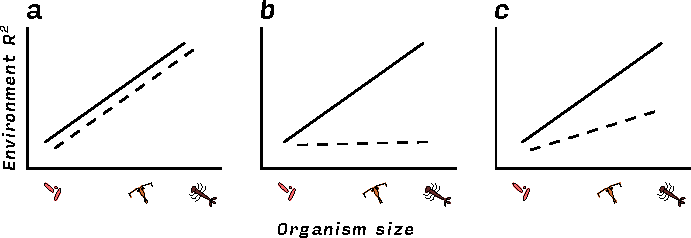
\includegraphics{../photos/hypotheses_illustration.pdf} \newpage

\textbf{Figure 2}

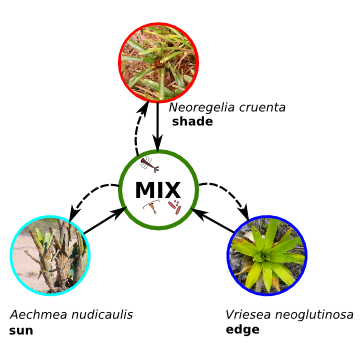
\includegraphics{../photos/design_illustration.pdf} \newpage

\textbf{Figure 3}

\begin{figure}
\centering
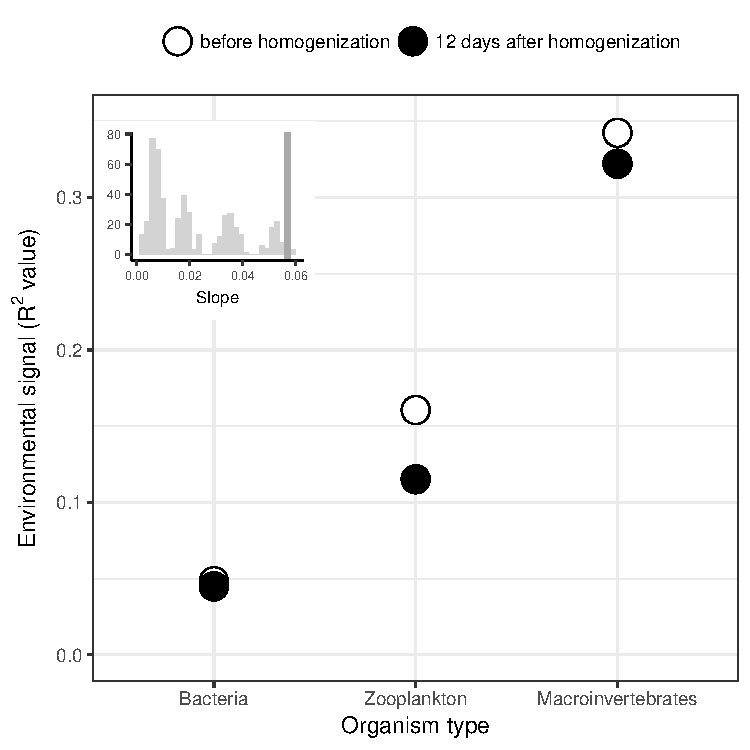
\includegraphics{../figures/r2_plot.pdf}
\caption{}
\end{figure}


\end{document}
